% make.tex
% Demonstration root file for building a LaTeX thesis
% Modified from ASR's 1999 mini.tex thesis builder
% 16-Jan-2009 ASR: Trimmed file down to a bare minimum template

\documentclass[a4paper,12pt,normalbib]{SLTCthesis}

\usepackage{graphicx,amsmath,amssymb,dcolumn,xspace,euscript}

\usepackage{geometry}
\geometry{
width=16cm,
height=24.5cm,
top=3cm,
headheight=14pt,
bindingoffset=2cm
}

\usepackage{cite}
%\usepackage{wrapfig,float,floatflt}
\usepackage{verbatim}
\usepackage{array}
\usepackage{calc}
\usepackage{url}
\usepackage{pdfpages}
\usepackage{enumitem}

\usepackage{rotating}
\usepackage{pdflscape}
\usepackage{pgfgantt}
\usepackage{xcolor}
\usepackage[utf8]{inputenc}

\definecolor{barblue}{RGB}{153,204,254}
\definecolor{groupblue}{RGB}{51,102,254}
\definecolor{linkred}{RGB}{165,0,33} 



\usepackage{fancyhdr}
\pagestyle{fancyplain}
\renewcommand{\chaptermark}[1]{\markboth{#1}{}}
\renewcommand{\sectionmark}[1]{\markright{\thesection\ #1}}
\lhead[\fancyplain{}{\bfseries\thepage}]%
      {\fancyplain{}{\bfseries\rightmark}}
\rhead[\fancyplain{}{\bfseries\leftmark}]%
      {\fancyplain{}{\bfseries\thepage}}

\lfoot[\fancyplain{}{}]%
      {\fancyplain{}{}}
\rfoot[\fancyplain{}{}]%
      {\fancyplain{}{}}
\cfoot{}

\newenvironment{myverbatim}[1]%
	{\linespread{0.9} \verbatiminput{#1}} 
	{}
\newenvironment{mytoc}%
	{\linespread{0.9} \verbatiminput{mytoc.tex}} 
	{}

% ASR.tex

\def\SKIP{\ifnum 0=1}
\def\NOSKIP{\ifnum 1=1}
\let\ENDSKIP=\fi

% \newcommand{}{}

\newcommand{\FIGS}{/home/asr/tex/thesis2/figs}
\newcommand{\HERE}{\textsf{\fbox{\bfseries $\Longleftarrow$ HERE!}}}

% Defns to produce JGR-style tables (this arithmetic should be
% generalised for arbitrary line spacing!)  See file 'ta5' for an
% 5-column table template example.

% settings for 11-point font:
\NOSKIP
% \def\tableline{\\[-11pt] \hline \\[-9pt]}
\def\tableline{\\[-10pt] \hline \\[-9pt]}
% \def\tablelinetop{\\[-5.5pt]\tableline}
\def\tableDline{\\[-5.5pt]\hline\hline\\[-8pt]}
\def\headvspA{\\[-19pt]}	% vert spacing above & below midline ruling
\def\headvspB{\\[-0pt]}
\ENDSKIP

% settings for 12-point font:
\SKIP
\def\tableline{\\[-12pt] \hline \\[-10pt]}
\def\tablelinetop{\\[-6pt]\tableline}
\def\headvspA{\\[-22pt]}	% vert spacing above & below midline ruling
\def\headvspB{\\[-1pt]}
\ENDSKIP


%------------------------------------------------------------------------
% Cortical defns



%------------------------------------------------------------------------
% Remote sensing defns

\newcommand{\JGR}{Journal of Geophysical Research}
\newcommand{\RSE}{Remote Sensing of the Environment}
\newcommand{\IJRS}{International Journal of Remote Sensing}

\newcommand{\micron}{$\mu$m}

\def\deg{\hbox{$^\circ$}}
\def\degC{\mbox{$\deg$\rm{C}}}

\def\Tx{\mbox{$T_x$}}
\def\Ts{\mbox{$T_s$}}
\def\Tc{\mbox{$T_c$}}
\def\Tair{\mbox{$T_{\rm air}$}}


\def\Tprice{\mbox{$T_{\rm Price}$}}
\def\BT{\mbox{\rm BT}}

\def\invcm{\mbox{${\rm cm}^{-1}$}}
\def\sqkm{\mbox{${\rm km}^2$}}
\def\sqm{\mbox{${\rm m}^2$}}

\def\epsx{\mbox{$\varepsilon_x$}}
\def\eps{\mbox{$\varepsilon$}}
\def\epsreq{\mbox{$\eps_{\rm req}$}}

\def\SST{\mbox{\rm SST}}

\newcommand{\mc}[2]{\multicolumn{#1}{c}{#2}}
% \def\mc#1#2{\multicolumn{#1}{c}{#2}}

\newcommand{\ul}[1]{\underline{#1}}

\newcommand{\rhoWV}{\rho_{\text{wv}}}
\newcommand{\rhoAir}{\rho_{\text{air}}}
\newcommand{\Rair}{R_{\text{air}}}
\newcommand{\Rwv}{R_{\text{wv}}}
\newcommand{\Mair}{M_{\text{air}}}
\newcommand{\Mwv}{M_{\text{wv}}}
\newcommand{\Tw}{T_{\text{w}}}
\newcommand{\cpair}{c_{\text{p,air}}}
\newcommand{\cpwv}{c_{\text{p,wv}}}
\newcommand{\mWV}{m_{\text{wv}}}
\newcommand{\ma}{m_{\text{a}}}
\newcommand{\DeltamWV}{\Delta\mWV}
\newcommand{\Lice}{L_{\text{ice}}}


\newcolumntype{.}{D{.}{.}{-1}}	% dcolumn: align on decimal point

%--------------------------
% Fix inter-line spacing when using the \intertext command by
% eliminating the \vskips either side of the \intertext argument.
% ASR: 8-Aug-2000

\makeatletter
\def\intertext{\@amsmath@err{\Invalid@@\intertext}\@eha}
\def\intertext@{%
  \def\intertext##1{%
    \ifvmode\else\\\@empty\fi
    \noalign{%
%     \penalty\postdisplaypenalty\vskip\belowdisplayskip%
      \penalty\postdisplaypenalty%
      \vbox{\normalbaselines
        \ifdim\linewidth=\columnwidth
        \else \parshape\@ne \@totalleftmargin \linewidth
        \fi
        \noindent##1\par}%
%     \penalty\predisplaypenalty\vskip\abovedisplayskip%
      \penalty\predisplaypenalty
   }%
}}
\makeatother
%--------------------------

\newcommand{\clearemptydoublepage}{\newpage{\pagestyle{empty}\cleardoublepage}}

\newcommand{\halothane}{CF$_3\cdot$CHClBr\xspace}
\newcommand{\cyclopropane}{C$_3$H$_6$\xspace}
\newcommand{\nitrousoxide}{N$_2$O\xspace}
\newcommand{\chloroform}{CHCl$_3$\xspace}
\newcommand{\ether}{CH$_3\cdot$CH$_2\cdot$O$\cdot$CH$_2\cdot$ CH$_3$\xspace}
\newcommand{\chloride}{Cl$^-$\xspace}
\newcommand{\sodium}{Na$^+$\xspace}
\newcommand{\potassium}{K$^+$\xspace}
\newcommand{\calcium}{Ca$^{2+}$\xspace}
\newcommand{\magnesium}{Mg$^{2+}$\xspace}
\newcommand{\GABAA}{GABA$_{\text{A}}$\xspace}
\newcommand{\NmOne}{N\!-\!1}
\newcommand{\muV}{$\mu$V}
\newcommand{\CMR}{$\text{CMR}_{\text{O}_2}$\xspace}
% \newcommand{\ul}[1]{\underline{#1}}
\newcommand{\dul}[1]{\underline{\underline{#1}}}
\newcommand{\asterisk}{\mbox{\textasteriskcentered}}
\newcommand{\bolddot}{\boldsymbol{\cdot}}
\newcommand{\boldLambda}{\mbox{\boldmath$\Lambda$}}
\newcommand{\boldGamma}{\mbox{\boldmath$\Gamma$}}
\newcommand{\boldsigma}{\mbox{\boldmath$\sigma$}}
\newcommand{\bolddelta}{\mbox{\boldmath$\delta$}}
\newcommand{\opentriangle}{\boldsymbol{\vartriangle}}
\newcommand{\opencirc}{\boldsymbol{\circ}}
\newcommand{\solidcirc}{\bullet}

\newcommand{\Eq}[1]{Eq.~(\ref{eq:#1})}
\newcommand{\Eqs}[1]{Eqs~(\ref{eq:#1})}
\newcommand{\Eqn}[1]{Equation~(\ref{eq:#1})}
\newcommand{\Fig}[1]{Fig.~\ref{fg:#1}}
\newcommand{\Figure}[1]{Figure~\ref{fg:#1}}

\newcommand{\closeup}{\vspace{-3ex}} % for displayed math eqns
\newcommand{\close}{\vspace{-5ex}}
\newcommand{\closei}{\vspace{-1ex}}
\newcommand{\closeii}{\vspace{-2ex}}

\newcommand{\etal}{\textit{et al.\xspace}}
\newcommand{\etalia}{\textit{et al}}

\newcommand{\Dh}{\Delta h}

\newcommand{\eq}{\:=\:}
\newcommand{\aeq}{\:&=\:}
\newcommand{\aaeq}{\:&&=\:}
\newcommand{\EQ}{\:\equiv\:}
\newcommand{\aEQ}{\:&\equiv\:}
\newcommand{\aaEQ}{\:&&\equiv\:}

\newcommand{\Approx}{\:\approx\:}
\newcommand{\TO}{\:\to\:}
% \renewcommand{\ln}{\log_e}
\newcommand{\RLH}{\:\rightleftharpoons\:}
\newcommand{\LRA}{\:\longrightarrow\:}
\newcommand{\lLRA}{\:\longleftrightarrow\:}
\newcommand{\LLRA}{\:\Longleftrightarrow\:}
\newcommand{\aLRA}{\:&\longrightarrow\:}

\def\SKIP{\ifnum 0=1}
\def\NOSKIP{\ifnum 1=1}
\let\ENDSKIP=\fi

\newcommand{\by}{\ensuremath{\times}}
\newcommand{\Matlab}{\textsc{Matlab}\xspace}

\newcommand{\omegalim}{{\omega_{\text{lim}}}}
\newcommand{\invN}{\textstyle \frac{1}{N}}
\newcommand{\betao}{\beta_{\mathrm{o}}}
\newcommand{\Io}{I_{\mathrm{o}}}
\newcommand{\he}{h_{e}}
\newcommand{\hi}{h_{i}}
\newcommand{\dhe}{\delta h_e}
\newcommand{\dhi}{\delta h_i}
\newcommand{\hei}{h_{e,i}}
\newcommand{\rms}{\text{rms}}
\newcommand{\heRms}{\he^{\text{rms}}}
\newcommand{\hiRms}{\hi^{\text{rms}}}
\newcommand{\heiRms}{h_{ei}^{\text{rms}}}
\newcommand{\heipmRms}{h_{ei}^{\pm\text{rms}}}
\newcommand{\heHatRms}{\widetilde{h}_e^{\text{rms}}}
\newcommand{\hiHatRms}{\widetilde{h}_i^{\text{rms}}}
\newcommand{\heiHatRms}{\widetilde{h}_{ei}^{\text{rms}}}
\newcommand{\heHat}{\hat{h}_e}
\newcommand{\hiHat}{\hat{h}_i}

\newcommand{\Iee}{I_{ee}(\he)}
\newcommand{\Iei}{I_{ei}(\he)}
\newcommand{\Iie}{I_{ie}(\hi)}
\newcommand{\Iii}{I_{ii}(\hi)}

\newcommand{\psiee}{\psi_{ee}(\he)}
\newcommand{\psiei}{\psi_{ei}(\hi)}
\newcommand{\psiie}{\psi_{ie}(\he)}
\newcommand{\psiii}{\psi_{ii}(\hi)}

\newcommand{\Jee}{J_{ee}}
\newcommand{\Jei}{J_{ei}}
\newcommand{\Jie}{J_{ie}}
\newcommand{\Jii}{J_{ii}}

\newcommand{\phie}{\phi_{e}(\he)}
\newcommand{\phii}{\phi_{i}(\he)}
\newcommand{\Phie}{\Phi_{e}}
\newcommand{\Phii}{\Phi_{i}}

\newcommand{\pee}{p_{ee}}
\newcommand{\pei}{p_{ei}}
\newcommand{\pie}{p_{ie}}
\newcommand{\pii}{p_{ii}}
\newcommand{\pjk}{p_{jk}}
\newcommand{\peeAv}{\langle p_{ee} \rangle}
\newcommand{\peiAv}{\langle p_{ei} \rangle}
\newcommand{\pieAv}{\langle p_{ie} \rangle}
\newcommand{\piiAv}{\langle p_{ii} \rangle}
\newcommand{\pjkAv}{\langle p_{jk} \rangle}

\newcommand{\geRest}{g_{e}^{\mathrm{rest}}}
\newcommand{\giRest}{g_{i}^{\mathrm{rest}}}
\newcommand{\heRest}{h_{e}^{\mathrm{rest}}}
\newcommand{\hiRest}{h_{i}^{\mathrm{rest}}}
\newcommand{\heiRest}{h_{e,i}^{\mathrm{rest}}}
\newcommand{\heRev}{h_{e}^{\mathrm{rev}}}
\newcommand{\hiRev}{h_{i}^{\mathrm{rev}}}
\newcommand{\taue}{\tau_{e}}
\newcommand{\taui}{\tau_{i}}
\newcommand{\gamme}{\gamma_{e}}
\newcommand{\gammi}{\gamma_{i}}
\newcommand{\gammiBar}{\overline{\gammi}}
\newcommand{\gammionLam}{\frac{\gammi}{\lambda}}
\newcommand{\Lee}{\Lambda_{ee}}
\newcommand{\Lei}{\Lambda_{ei}}
\newcommand{\Lie}{\Lambda_{ie}}
\newcommand{\Lii}{\Lambda_{ii}}
\newcommand{\Neeb}{N_{ee}^{\beta}}
\newcommand{\Neib}{N_{ei}^{\beta}}
\newcommand{\Nieb}{N_{ie}^{\beta}}
\newcommand{\Niib}{N_{ii}^{\beta}}
\newcommand{\Neea}{N_{ee}^{\alpha}}
\newcommand{\Neia}{N_{ei}^{\alpha}}
\newcommand{\Ge}{G_e}
\newcommand{\Gi}{G_i}
\newcommand{\ddt}{\frac{d}{dt}}
\newcommand{\col}[2]{\left[{#1 \atop #2} \right]}
\newcommand{\Det}[1]{\text{Det}\!\left( #1 \right)}
\newcommand{\Tr}[1]{\text{Tr}\!\left( #1 \right)}
\newcommand{\var}[1]{\text{var}\!\left( #1 \right)}

\newcommand{\euR}{{\EuScript{R}}}
\newcommand{\euS}{{\EuScript{S}}}
\newcommand{\Se}{{\EuScript{S}}_{e}(\he)}
\newcommand{\Si}{{\EuScript{S}}_{i}(\hi)}
\newcommand{\Semax}{{\EuScript{S}}_e^{\max}}
\newcommand{\Simax}{{\EuScript{S}}_i^{\max}}


%Laplace transform L
\newcommand{\LapL}{\mathscr{L}}
\usepackage{mathrsfs}


%\includeonly{titlepage,abstract,preface,acronyms,ch1,ch2,ch3,ch4,ch5,ch6,ch7,ch8,ch9,ch10,appendixA,appendixB}

% \includeonly{titlepage,abstract,preface,acronyms,ch1}

\begin{document}

\begin{titlepage}
\begin{center}

\vspace*{1cm}

\textsf{\Huge\bfseries{%
Supercapacitor-Assisted Temperature
Modification Apparatus (SCATMA)
and
Fast Supercapacitor Charger\\
}}

\vfill

\textsf{\large%
	A thesis \\[1ex]
	submitted in partial fulfilment\\[1ex]
	of the requirements for the degree\\[1ex]
	of\\[1ex]
\textbf{\Large Bachelor of Science}\\[1ex]
	in Engineering \\[1ex]
	in Electronics and Power Systems \\[1ex]
		at\\[1ex]
		\textbf{\Large Sri Lanka Technological Campus}\\[1ex]
	by  \\[2ex]
}
\textsf{\LARGE\bfseries{Nicoloy Gurusinghe}}\\

\vfill


\includegraphics[height=6.5cm]{_figs/SLTC LOGO.png}

 2021\\
%\bf{\large{The University of Waikato}}
\end{center}
\end{titlepage}

\clearemptydoublepage
\newpage


%
\pagenumbering{roman}
%

\chapter*{Abstract}
\addcontentsline{toc}{chapter}{Abstract}

This thesis presents the design and development of the supercapacitor assisted ``instant" water heating system as well as a new power converter topology to fast charge a supercapacitor bank.

 Delayed delivery of hot water in domestic water heating systems waste over 15 million cubic metres of treated water per annum in New Zealand. The patent pending supercapacitor assisted temperature modification apparatus~(SCATMA), solves this problem by using pre-stored supercapacitor energy. These supercapacitors deliver short-term high-power bursts into heater coils placed in the final half meter of pipe connecting the faucet.  During a period of less than a minute, 100--200~Wh of energy is released to the heater coil at a rate between 10--20~kW.


Based on the cost constraints of a commercial system and the regulatory authority requirements, a supercapacitor-only solution becomes prohibitively expensive. A review of current state-of-the-art energy storage systems show that no battery chemistry can withstand the associated charge-discharge cycles to reach the expected service life of 5--10 years. While developing the unique two-stage fast supercapacitor charger, a battery-supercapacitor hybrid system was developed for SCATMA as a commercially viable solution for rapid water heating.   
 
Dividing a supercapacitor bank into three parts and circulating them through a `charge-idle-discharge' sequence was already investigated for the surge resistant uninterrupted power supply. The effectiveness of this technique mandates fast supercapacitor charging. The proposed new charger achieves fast charging by using a high voltage source to overcome the five time constant charging time and a series coupled inductor to charge the  capacitor bank by dividing it into two parts. One part is charged using an over-voltaged dc source with capacitor bank terminal voltage monitoring and the other part is charged by the coupled-inductor using the energy stored in the inductor.

 






%
%\clearpage
%\chapter*{Acknowledgements}
\addcontentsline{toc}{chapter}{Acknowledgements}

I wish to acknowledge with considerable gratitude the contributions
and help received from a host of colleagues:

%
\tableofcontents 
%
\addcontentsline{toc}{chapter}{List of Figures}
\addcontentsline{toc}{chapter}{List of Tables}
\listoffigures
\begingroup
\let\clearpage\relax
\listoftables
\endgroup

%
\clearpage

\chapter*{Acronyms and Abbreviations}
\addcontentsline{toc}{chapter}{Acronyms and Abbreviations}
%----------------------------------------------------------------
% Set width of left column (the acronyms) to appropriate value

\newcommand{\WidestWord}{AP5, APV}  % <<-- longest word in left col

\newlength{\tmpleft}
\settowidth{\tmpleft}{\WidestWord}

% Compute appropriate width for right column
\newlength{\tmpright}
\setlength{\tmpright}{\linewidth - \tabcolsep - \tmpleft}
%----------------------------------------------------------------

\begin{tabular*}{\linewidth}{p{\the\tmpleft}p{\the\tmpright}}
%
1D, 2D & one-dimensional, two-dimensional \\
AMPA   & $\alpha$-amino-3-hydroxy-5-methyl-4 isoxazole propionic acid
	(a neurotransmitter associated with the fast-decaying ``early''  
	current in the excitatory postsynapse; cf. NMDA)\\
AP5, APV    & 2-amino-5-phosphonovalerate (an NMDA-blocking agent)\\
CMR & cerebral metabolic rate \\
DE	& differential equation\\
ECoG   & electrocorticogram (brain activity recorded via electrodes
	attached directly to the cerebral cortex; cf. EEG)\\
EEG    & electroencephalogram (brain activity recorded via scalp
	electrodes; cf. ECoG)\\
EPSC   & excitatory postsynaptic current \\
EPSP   & excitatory postsynaptic potential \\
DFT  & discrete Fourier transform \\
GABA  & $\gamma$-aminobutyric acid (an inhibitory neurotransmitter)\\
GHK & Goldman--Hodgkin--Katz formula for membrane voltage \\
IPSC   & inhibitory postsynaptic current \\
IPSP   & inhibitory postsynaptic potential \\
LOC	& loss of consciousness \\
MAC & minimum anaesthetic concentration (a standard measure of anaesthetic
potency) \\
MEG & magnetoencephalogram (brain activity recorded via magnetic-field
	probes) \\
NOS & nitric oxide synthase (an enzyme that catalyzes production of NO,
	nitric oxide) \\
ODE	& ordinary differential equation \\
OU  & Ornstein--Uhlenbeck (random process describing the 
	velocity of a Brownian particle) \\
PDE	& partial differential equation \\
PDF	& probability density function \\
PSP    & postsynaptic potential \\
SDE	& stochastic differential equation (Langevin equation) \\
rms    & root-mean square \\
%
\end{tabular*}

                                                                                                                           


 \setcounter{page}{0}
%
\pagenumbering{arabic} % sets page# = 1
\clearemptydoublepage
%-------------------------------------------------------------------
\chapter{\textbf{"Instantaneous" Water Heating}}
\chaptermark{ water heating}
%-------------------------------------------------------------------

\section{Scope}

The scope of this thesis is to present the results obtained in the PhD project ``SCATMA and supercapacitor-fast charger" undertaken by the author from March 2013 to January 2016. Most of the scientific findings of this project have been published in the form of peer reviewed conference and journal papers and a patent application. 

\section{Background and Motivation}

The inventions  developed by this group 
5
 include

\begin{itemize}
	
	\item SCALDO - SC-assisted low-dropout regulator - a high efficient dc--dc converter technique using low dropout regulators\cite{SCALDO_patent}
	\item SCASA - SC-assisted surge absorber - a technique developed to absorb power-line surges using SCs\cite{SCASA_patent}
	\item SRUPS - surge resistant uninterrupted power supply - a batteryless uninterrupted power supply~(UPS) technique capable of absorbing power line surges\cite{SRUPS:11}
	\item SCATMA - SC-assisted temperature modification apparatus - an ``instant" liquid flow heating technique based on stored energy\cite{SCATMA:14}
	\item SCAHDI - SC-assisted high density inverter - a SC technique to improve efficiency and packing density of a high power inverter
	
\end{itemize}

The initial SCATMA concept was developed in late 2012. 


\section{``Instantaneous'' Water Heating Problem}

Delayed hot water delivery in domestic water heating systems is a worldwide problem. A typical domestic hot water system will have a delay of around $5$--$30$~s on average depending on the distance of the tap from the central hot-water tank. 
There are a few commercial solutions proposed to address this problem. These solutions include 

\subsection{Requirements}

The above power and energy requirement is estimated for the worst case.

\begin{itemize}
	
	\item Electrical safety and isolation\\
	Due to safety concerns, a power source over 60 V cannot be utilized because of the low voltage requirements to prevent electrical shock. If mains power is used directly, galvanic isolation via a transformer supplying less than 60 V (rms) may be required as the high-power heater coil is directly in contact with the flowing water\cite{AS/NZSIWH04}.
	
	\item Domestic installation regulations\\
	Domestic subcircuits are protected using overcurrent protection devices\cite{AS/NZSRCD11(c)}. The maximum power rating for a domestic subcircuit will be 6.9 kW even if a 30 A dedicated sub-circuit is available. Therefore it is impractical for an existing electrical subcircuit to solely deliver this power.
	
\end{itemize}



...
% \pagestyle{empty}
% \begin{landscape}
% \begin{table}[htbp]
% \begin{center}
% \begin{tabular}{llll}
% ...
% \end{tabular}
% \end{center}
% \end{table} 
% \end{landscape}
% \pagestyle{plain}

\begin{sidewaystable}
  \centering
  \caption{A rotated table}
  	\begin{tabular}{clccc}
		\tableDline
		Parameters                            & minimum & average & maximum \\
		\tableline
		Water flow rate (litres/min)            & $4$   & $6$     & $8$  \\
		Delay in centrally heated hot water (s) & $5$   & $15$    & $30 $ \\ 
		Required temperature rise ($\degC$)     & $20$  & $30$    & $40$  \\ 
		Required energy (Wh)                    & $7.8$ & $52.5$  & $186.7$  \\
		Required power (kW)                     & $5.6$ & $12.6$  & $22.4$  \\  
			%
			\tableDline
		\end{tabular}
  \label{tab:test}
\end{sidewaystable}

\begin{table}[t]
	\centering
	\caption[Typical domestic ``instant"-water heating problem specifications]
	{Typical domestic ``instant"-water heating problem specifications}
	\label{ta:SCATMA_for_LWH}
	%
	\begin{tabular}{clccc}
		\tableDline
		Parameters                            & minimum & average & maximum \\
		\tableline
		Water flow rate (litres/min)            & $4$   & $6$     & $8$  \\
		Delay in centrally heated hot water (s) & $5$   & $15$    & $30 $ \\ 
		Required temperature rise ($\degC$)     & $20$  & $30$    & $40$  \\ 
		Required energy (Wh)                    & $7.8$ & $52.5$  & $186.7$  \\
		Required power (kW)                     & $5.6$ & $12.6$  & $22.4$  \\  
			%
			\tableDline
		\end{tabular}
	\end{table}














%-----------------------------------------------------------------------  % contains the 

%-------------------------------------------------------------------
\chapter{\textbf{SCATMA Basics and Requirements}}
\label{ch:basics}
% \chaptermark{Fourier Transform Theory}
%-------------------------------------------------------------------

This chapter presents the instant water heating problem, the SCATMA solution and the main concerns in selecting an energy storage medium for this application. 

\section{Heating Still and Flowing Water}
% \sectionmark{Continuous-Time Representation}

The amount of energy $E$ [in J] required to raise the temperature of $l$ litres of water inside a perfectly insulated container by $\Delta\theta$~[$\deg$C] is 
%
\begin{equation}
\label{eq:stil_energy}
  E\eq\rho lC\Delta\theta
\end{equation}
%
where $\rho$ is the density of water [kg\,L$^{-1}$], $C$ is the specific heat capacity of water~[J\,kg$^{-1}$\,$\deg$C$^{-1}$].
If the temperature rise $\Delta\theta$ is to occur within time $\Delta T$, the required average heating power $P$ can be calculated as
%
\begin{equation}
\label{eq:still_power}
    P\eq\frac{E}{\Delta T}\eq\frac{\rho lC\Delta\theta}{\Delta t} 
\end{equation}
%
where no losses are assumed at the source or in the power transfer path.
Inserting Eq.(\ref{eq:stil_energy}) gives
%
\begin{equation}
\label{eq:still_power_rearrange}
P\eq\frac{l}{\Delta t}\rho C\Delta\theta\eq Q\rho C\Delta\theta
\end{equation}
%
where $Q$ is the water flow rate [Lmin$^{-1}$]. This equation describes heating a flow of water with~$100\%$ heat transfer efficiency at the heating element surface.
%




%-------------------------------------------------------------------
\subsection{Electric Kettle Example}

Take the static example of a 230~V, 2.3~kW rated 4-litre electric kettle. It takes 9.7 min to raise the temperature of 4~L of water from 20$\deg$C room temperature to 100$\deg$C. This result follows form Eq.~(\ref{eq:still_power}),
%
\begin{equation}
\label{eq:kettle _still}
2300~\text{W} \eq \frac{(1~\text{kg\,L}^{-1})(4200~\text{J\,kg}^{-1}\,\deg \text{C}^{-1}) (80\deg \text{C}}{\Delta t})~~~ \implies~~~ \Delta t \eq 9.74~ \text{min}
\end{equation}



If the same power input is applied to water flowing inside a perfectly insulated tube, then the maximum permissible flow rate for the same temperature rise is $0.41$~L\,min$^{-1}$,
%
\begin{equation}
\label{eq:kettle _flow}
2300~\text{W}\eq\left(\frac{4~\text{L}}{9.74~\text{min}}\right)\rho C\,(80\deg \text{C})~~~\implies ~~~ Q\,\eq\,0.41~\text{L\,min}^{-1}
\end{equation}


Similarly if the temperature rise is halved to 40$\deg$C then the maximum flow rate for the same heater power would be doubled to 0.81~L\,min$^{-1}$. If the flow rate needs to be increased ten-fold to 8~Lmin$^{-1}$ for the same 40$\deg$C temperature rise, then a ten-fold higher power source of 23~kW is required. 

\begin{figure}[t]
	\centering
	 \resizebox{16cm}{!}{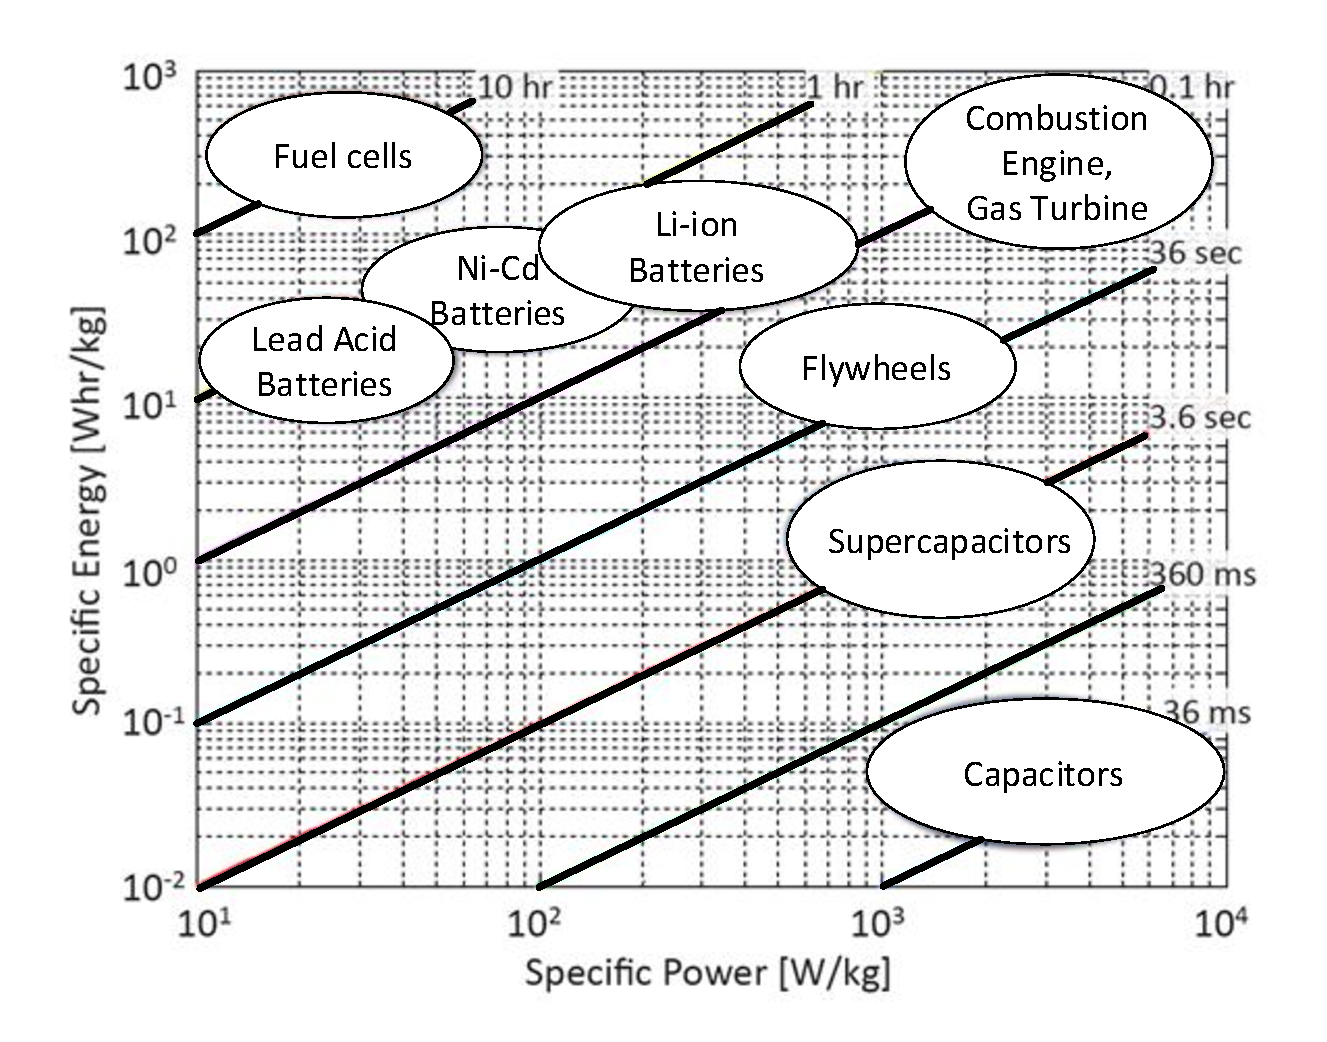
\includegraphics[draft=false]{_figs/th_ragone_vco}}
	%\includegraphics[draft=false]{_figs/Ragone_plot}
	\caption[ Ragone plot]
		{%
		\label{fg:Ragone_plot}
		\centering
		Ragone plot of various energy storage/propulsion devices and their ``charge" times.  Adapted from US Defense Logistics Agency Report~\cite{Obey:09} 
	}
\end{figure}

  % 
%-------------------------------------------------------------------
\chapter{\textbf{SCATMA Prototype Design}}
\label{ch:prototype}
%-------------------------------------------------------------------

%-----------------------------------------------------------------------

\section{Implementation of a Prototype System}

\subsection{Implementation}
Given the advantage of a series-hybrid configuration in Fig.~\ref{fg:series_hybrid_block}, the first implementation and related tests  were carried out based on the simplified block diagram of Fig.~\ref{fg:series_hybrid_block}. 


%-----------------------------------------------------------------------
\begin{figure}[b]
	\centering
	\resizebox{14cm}{!}{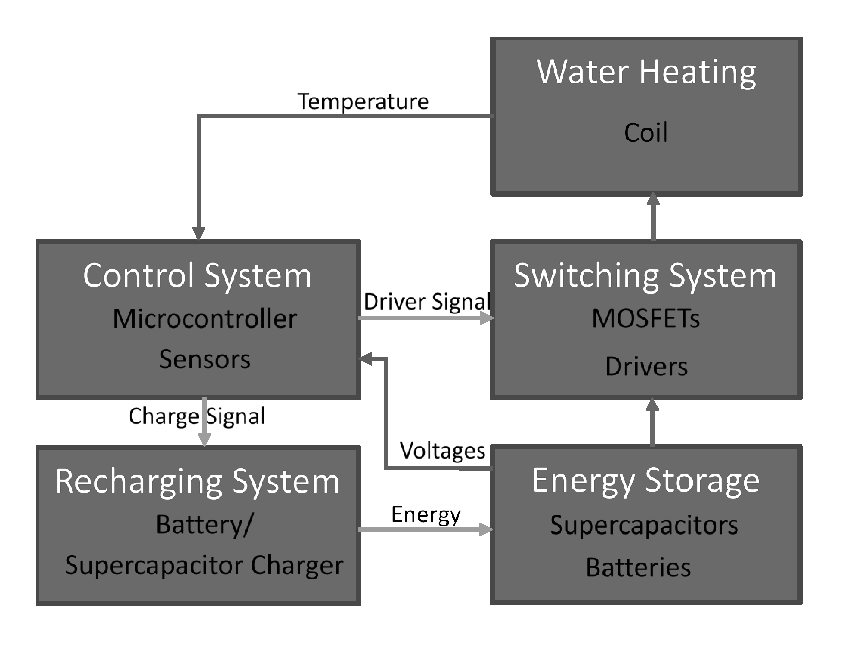
\includegraphics[draft=false]{_figs/series_hybrid_block.pdf}}
	%\includegraphics[draft=false]{_figs/Ragone_plot}
	\caption[Simplified block diagram of the hybrid-series system.]
	{%
		\label{fg:series_hybrid_block}
		\centering
		Simplified block diagram of the series-hybrid system.}
\end{figure}
%-----------------------------------------------------------------------
  % 
%-------------------------------------------------------------------
\chapter{\textbf{Fast Supercapacitor Charger for SCATMA}}
\label{ch:Charger_basics}
%-------------------------------------------------------------------

\section{Fast Charging Requirement in SCATMA}
As described in previous chapters, ``instant" water heating requires stored energy that can be delivered at a fast rate. The hybrid solution based on a SC/battery series-hybrid arrangement as described in Chapter~\ref{ch:prototype} has the major drawback that the size of the required energy storage is too big. Compared with SCs, batteries have a very short cycle life~(one million deep discharge cycles for SCs vs a maximum of 1000--2000 for batteries\cite{Schneuwly:00}). 

%-------------------------------------------------------------------
\subsection{Energy Balance}
Based on the average specifications of ``instant" water heating, 100--150~Wh of energy is required for the 30~s period of operation. A SC bank providing up to 50~Wh is feasible based on cost and size. Possible options for the rest of the energy requirement are

\begin{enumerate}
	\item to draw more than 10 A from the mains supply for a short period of time without overloading the wiring or tripping the protective circuit breaker.  
	\item to draw the nominal 2.3~kW from the mains supply. This can be used for the time after the mains supply has had its 10 A supply exceeded by the previous option.
	\item to store energy by a cheaper alternative than SCs (such as a battery). Such a store can have a lower power density but a higher energy density than SCs.
\end{enumerate}



Given the availability of these options the problem lies in how this energy can be delivered to the load with galvanic isolation and at the required 15--18~kW average power level. For both of these conditions to be satisfied, a SC bank circulation technique first proposed for surge resistant uninterrupted power supply~(SRUPS)\cite{SRUPS:11, Madawala:2007} is used.

\subsection {SRUPS}    

 The first scenario is for charging a capacitor fully discharged from a voltage source at the capacitor rated voltage. This method loses the same amount of energy as stored in the capacitor in the lumped resistor irrespective of the value of the total resistance of the charging path. The second scenario is charging a partially discharged capacitor from a voltage source at the capacitor rated voltage. The losses are dependant on the start factor $n$ and they vary as seen in, the best charging efficiency is achieved when $E_C - E_R$ maximises. That is when the first derivative of $E_C - E_R$ with respect to $n$ becomes zero:


\begin{figure}[h]
	\centering
	\resizebox{16cm}{!}{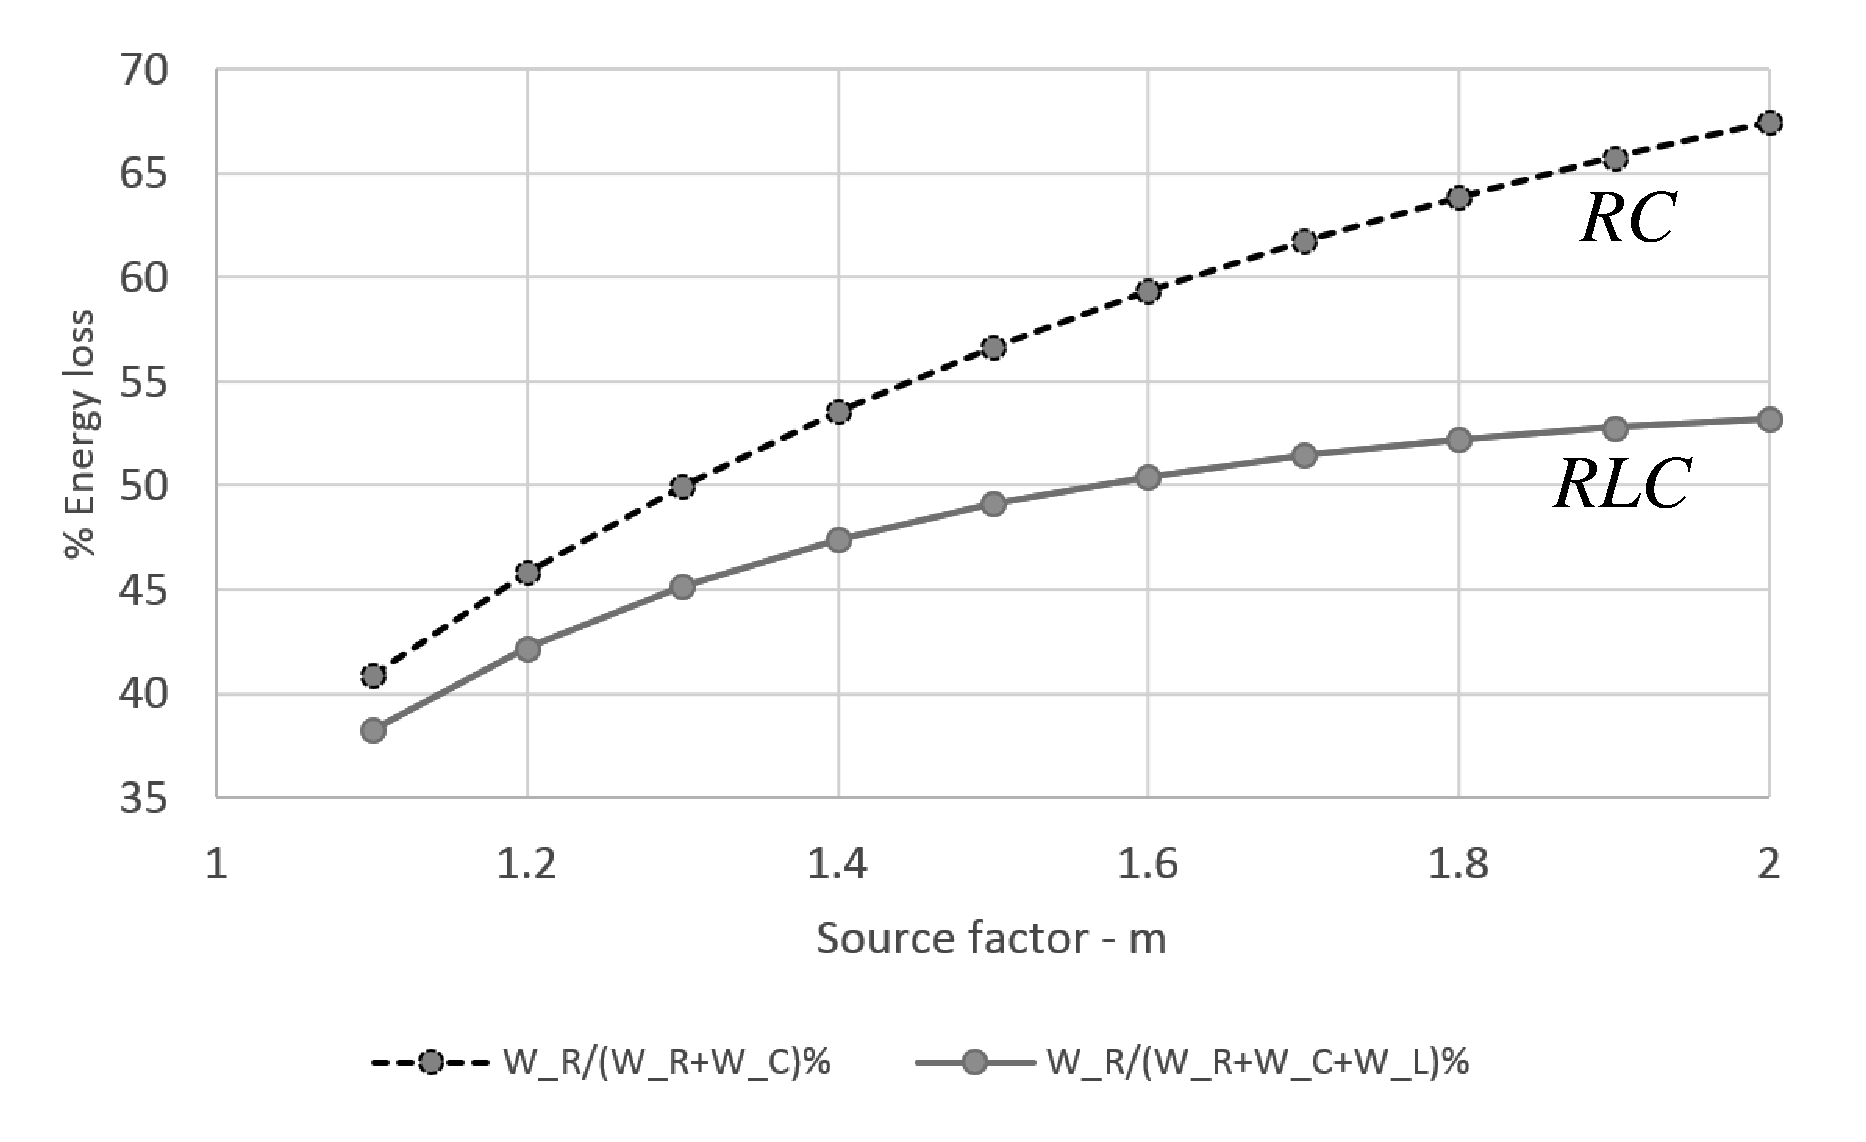
\includegraphics[draft=false]{_figs/RC_RLC_advantage_sim.pdf}}
	%\includegraphics[draft=false]{_figs/Ragone_plot}
	\caption[Efficiency improvement of a $RLC$ system]
	{%
		\label{fg:RC_RLC_advantage_sim}
		\centering
		Efficiency improvement of a $RLC$ system over a $RC$ system for $m$-times charging ($C = 310~$F$, L = 2$ mH, $R = 50~$m$\Omega, V_C = 2.7 $V, $n = 0.3$)}
\end{figure}





  % 
%-------------------------------------------------------------------
\chapter{\textbf{Fast Charger Design}}
\label{ch:Charger_design}
%-------------------------------------------------------------------

It was seen in Chapter\ref{ch:Charger_basics}, that the fast charging requirement of applications like SCATMA and SRUPS are unique. 

\begin{itemize}
	\item Ability to extract the energy stored in the above mentioned inductor to charge a separate part of the same capacitor bank
	\item Ability to use a higher voltage to charge one part of the capacitor
\end{itemize}

\begin{align*}
L_a \aeq L_1 + L_2 + 2M,\\[1ex]
L_b \aeq L_1 - L_2 - 2M.
\end{align*}

By solving these two equations;

\begin{align}
\label{eq:La_Lb_M}
L_1 + L_2 \eq \frac{L_a +L_b}{2}~~~and~~~M\eq\frac{L_a - L_b}{4}.
\end{align}

The coupling coefficient~($k$) can be found using the following equation

\begin{align}
\label{eq:La_Lb_k}
k \eq \sqrt{\frac{M^2}{L_1L_2}}.
\end{align}

From the practical measurements the following values were obtained; $L_1=1.26~\text{mH},~ L_2\eq1.48~\text{mH},~l_p=19.9~\mu\text{H},~L_a\eq5.47~\text{mH}~and~L_b\eq31.21~\mu\text{H}$. Hence $L_1 + L_2\eq1.26 + 1.48~\text{mH}\eq 2.74~\text{mH}$. $L_1 + L_2$ can be obtained using $L_a ~\text{and}~ L_b$ according to Eq.~\ref{eq:La_Lb_M}. 

Mutual inductance can be calculated from Eq.~\ref{eq:La_Lb_M} 
\begin{align*}
M \eq \frac{5.47 - 0.031}{4}~\text{mH} \eq 1.36~\text{mH}.  
\end{align*}


The coupling coefficient calculated according to Eq.~\ref{eq:La_Lb_k}

\begin{align*}
k \eq \sqrt{\frac{1.36^2}{1.26 \times 1.48}}~~\implies~~ k \eq 0.995.
\end{align*}

Sample gantt chart:




\begin{ganttchart}{1}{24}
\gantttitle{Project Name}{24} \\
\gantttitlelist{1,2,3,4,5,6,7,8,9,10,11,12}{2} \\
\ganttbar{Proposal Submission}{1}{1}\\
\ganttbar{Project...}{2}{3}\\
\ganttmilestone{Mid Review}{14} \\
\ganttbar{Final Task}{22}{24}
\end{ganttchart}



%%%%%%%%%%%%%%%%%%%%%%%%%%%%%%%%%%%%%%%%%%%%%%%%%%%%%%%%%%%%%%%%%%%%%%%%%%%%%%%%%%%%%%%%%%%%%%%%%%%%%%%%%%%%%%%%%%%%%%%%%%%%%%%%%%%%%%%%%%%%%%%  % 
%-------------------------------------------------------------------
\chapter{\textbf{Conclusions and Future Work}}
\label{ch:conclude_future}
%-------------------------------------------------------------------

\section{Summary and Conclusion}

The analysis on the ``instantaneous" water heating problem revealed the specifications for SCATMA.
\noindent Having identified pre-stored energy as the only solution to the problem, and the limitations of each device, the closest practical implementation is a hybridization of SCs with cheap lead-acid batteries. 


This method requires capacitor voltage monitoring to avoid overcharging. The converter works in transient mode and PFC is achieved without using any additional components~(by the same switch used in the primary side). The simulation and experimental results on the prototype design suggests

\begin{itemize}
	\item The equivalent charging rate can be calculated based on the primary and secondary peak currents
	\item The converter design has inherent transient mode power factor correction capability
	\item The design is energy limited based on the transformer design and component selection
\end{itemize}


\section{Future Work}

Battery Storage Optimisation:
o	The battery storage configuration requires more investigation. 

\noindent Supercapacitor Optimisation:
o	The current system is showing that a number of the specifications are being reached, or are close to being reached. Additional supercapacitors will be introduced to the system, to hit all targets (including worst case scenarios). 































  % 

\clearpage									% needed to get page no. 
\addcontentsline{toc}{chapter}{References}  % in TOC correct
\bibliographystyle{IEEEtran}
\bibliography{thesis_bib}

\chapter*{\textbf{Appendix A: Publications}}
\addcontentsline{toc}{chapter}{Appendix A}

\label{ap:publications}
%----------------------------------------------------------------------

Appendix A is contains a list of publications made as part of this project i.e. conference papers,
journal papers and patent application. Excluding Appendix A.1 all the rest is original contributions by the author during the PhD.\\

\begin{enumerate}[label=\bfseries A \arabic*.]
\item N. Kularatna, Fluid temperature modification apparatus,``WO2014/189389 A1, International Patent application PCT/NZ2014/000092.\\

\item N. Kularatna, A. Gattuso, N. Gurusinghe, T. Jayasuriya, J. Du Toit, ``Pre-stored supercapacitor energy as a solution for burst energy requirements in domestic in-line fast water heating systems,” in Proc of IECON 2014,USA, Nov. IEEE, 2014.\\

\item N. Gurusinghe, N. Kularatna, D. A. Steyn-Ross, ``Essential Physics for "instantaneous" delivery of hot water: SCATMA," in proc of NZIP 2015, NZ, Jul, 2015.\\

\item N. Gurusinghe, N. Kularatna, S. A. Charleston, W. H. Round and J. Fernando, ``Hybridisation techniques in Supercapacitor Assisted Temperature Modification Apparatus for inline water heating," in Proc of IECON 2015, JAPAN, Nov. IEEE, 2015.\\

\item N. Gurusinghe, N. Kularatna, W. H. Round and D. A. Steyn-Ross ``Design approaches for fast supercapacitor chargers for applications like SCATMA, SRUPS” in proc of APEC 2016, USA, Mar. IEEE, 2016.\\

\item N. Kularatna, N. Gurusinghe, ``Electrical energy charging apparatus," New Zealand Patent application P31578NZ00.\\


\end{enumerate}

	
	
	
	

	
	




  % 

\end{document}

